        \documentclass[crop,tikz, border=5pt]{beamer}
        
        \usepackage{pgf}
        \usepackage{tikz}
        \usepackage{amsmath, amssymb}
        \usetikzlibrary{arrows.meta}
        \usetikzlibrary{arrows}
        \usetikzlibrary{calc}
        \usetikzlibrary{shapes}
        \usepackage[utf8]{inputenc}
        \usetikzlibrary{calc}
        \usetheme{default}
        \usefonttheme{professionalfonts}
        \setbeamertemplate{navigation symbols}{}
        \setbeamerfont{frametitle}{series=\bfseries}
    
        \begin{document}
        \begin{frame}
        \frametitle{Dijkstra's Algorithm : Input}
        \begin{center}
        
        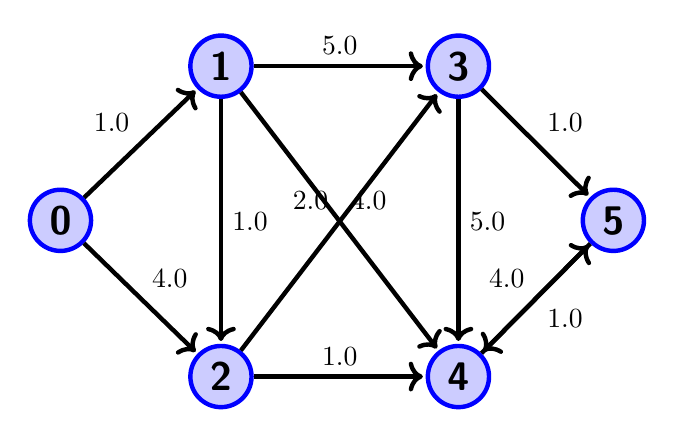
\begin{tikzpicture}[shorten >=1pt, auto, node distance=3cm, ultra thick,
        node_style/.style={circle,draw=blue,fill=blue!20!,font=\sffamily\Large\bfseries},
        selected_node_style/.style={circle,draw=blue,fill=yellow!20!,font=\sffamily\Large\bfseries},
        edge_style/.style={draw=black, ultra thick,->},
        selected_edge_style/.style={draw=yellow, ultra thick,->}]
        
        \node [node_style,label={[text=blue]10:$$}](n1) at (3.471,3.511) {0};
    
        \node [node_style,label={[text=blue]10:$$}](n2) at (5.509,5.469) {1};
    
        \node [node_style,label={[text=blue]10:$$}](n3) at (5.509,1.527) {2};
    
        \node [node_style,label={[text=blue]10:$$}](n4) at (8.525,5.469) {3};
    
        \node [node_style,label={[text=blue]10:$$}](n5) at (8.525,1.527) {4};
    
        \node [node_style,label={[text=blue]10:$$}](n6) at (10.493,3.511) {5};
    
        \draw [edge_style] (n5) edge node{4.0} (n6);
    
        \draw [edge_style] (n6) edge node{1.0} (n5);
    
        \draw [edge_style] (n2) edge node{1.0} (n3);
    
        \draw [edge_style] (n1) edge node{4.0} (n3);
    
        \draw [edge_style] (n4) edge node{1.0} (n6);
    
        \draw [edge_style] (n2) edge node{4.0} (n5);
    
        \draw [edge_style] (n3) edge node{2.0} (n4);
    
        \draw [edge_style] (n1) edge node{1.0} (n2);
    
        \draw [edge_style] (n2) edge node{5.0} (n4);
    
        \draw [edge_style] (n3) edge node{1.0} (n5);
    
        \draw [edge_style] (n4) edge node{5.0} (n5);
    
        \end{tikzpicture}
    
        \end{center}
        \end{frame}
        
            \begin{frame}
            \frametitle{Dijkstra's Algorithm : Iteration 1 }
            \begin{center}
            
        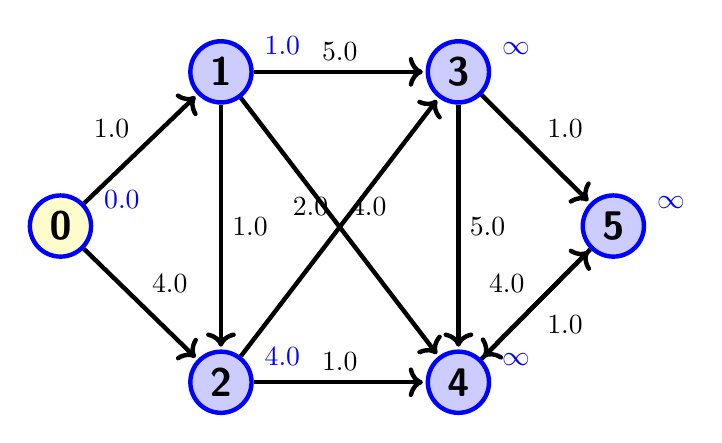
\begin{tikzpicture}[shorten >=1pt, auto, node distance=3cm, ultra thick,
        node_style/.style={circle,draw=blue,fill=blue!20!,font=\sffamily\Large\bfseries},
        selected_node_style/.style={circle,draw=blue,fill=yellow!20!,font=\sffamily\Large\bfseries},
        edge_style/.style={draw=black, ultra thick,->},
        selected_edge_style/.style={draw=yellow, ultra thick,->}]
        
        \node [selected_node_style,label={[text=blue]10:$0.0$}](n1) at (3.471,3.511) {0};
    
        \node [node_style,label={[text=blue]10:$1.0$}](n2) at (5.509,5.469) {1};
    
        \node [node_style,label={[text=blue]10:$4.0$}](n3) at (5.509,1.527) {2};
    
        \node [node_style,label={[text=blue]10:$\infty$}](n4) at (8.525,5.469) {3};
    
        \node [node_style,label={[text=blue]10:$\infty$}](n5) at (8.525,1.527) {4};
    
        \node [node_style,label={[text=blue]10:$\infty$}](n6) at (10.493,3.511) {5};
    
        \draw [edge_style] (n5) edge node{4.0} (n6);
    
        \draw [edge_style] (n6) edge node{1.0} (n5);
    
        \draw [edge_style] (n2) edge node{1.0} (n3);
    
        \draw [edge_style] (n1) edge node{4.0} (n3);
    
        \draw [edge_style] (n4) edge node{1.0} (n6);
    
        \draw [edge_style] (n2) edge node{4.0} (n5);
    
        \draw [edge_style] (n3) edge node{2.0} (n4);
    
        \draw [edge_style] (n1) edge node{1.0} (n2);
    
        \draw [edge_style] (n2) edge node{5.0} (n4);
    
        \draw [edge_style] (n3) edge node{1.0} (n5);
    
        \draw [edge_style] (n4) edge node{5.0} (n5);
    
        \end{tikzpicture}
    
            \end{center}
            \end{frame}
        
            \begin{frame}
            \frametitle{Dijkstra's Algorithm : Iteration 2 }
            \begin{center}
            
        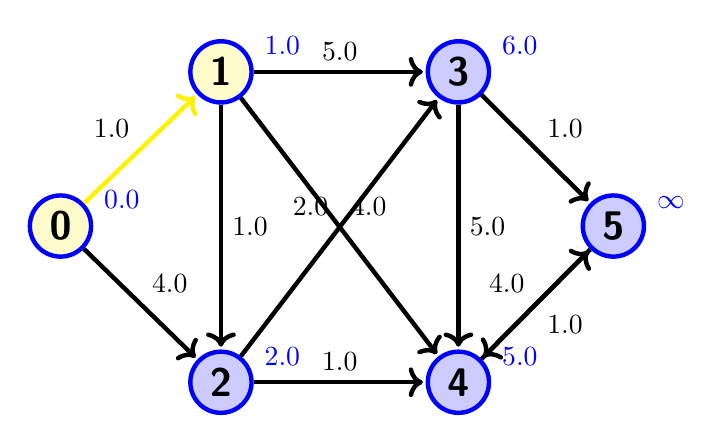
\begin{tikzpicture}[shorten >=1pt, auto, node distance=3cm, ultra thick,
        node_style/.style={circle,draw=blue,fill=blue!20!,font=\sffamily\Large\bfseries},
        selected_node_style/.style={circle,draw=blue,fill=yellow!20!,font=\sffamily\Large\bfseries},
        edge_style/.style={draw=black, ultra thick,->},
        selected_edge_style/.style={draw=yellow, ultra thick,->}]
        
        \node [selected_node_style,label={[text=blue]10:$0.0$}](n1) at (3.471,3.511) {0};
    
        \node [selected_node_style,label={[text=blue]10:$1.0$}](n2) at (5.509,5.469) {1};
    
        \node [node_style,label={[text=blue]10:$2.0$}](n3) at (5.509,1.527) {2};
    
        \node [node_style,label={[text=blue]10:$6.0$}](n4) at (8.525,5.469) {3};
    
        \node [node_style,label={[text=blue]10:$5.0$}](n5) at (8.525,1.527) {4};
    
        \node [node_style,label={[text=blue]10:$\infty$}](n6) at (10.493,3.511) {5};
    
        \draw [edge_style] (n5) edge node{4.0} (n6);
    
        \draw [edge_style] (n6) edge node{1.0} (n5);
    
        \draw [edge_style] (n2) edge node{1.0} (n3);
    
        \draw [edge_style] (n1) edge node{4.0} (n3);
    
        \draw [edge_style] (n4) edge node{1.0} (n6);
    
        \draw [edge_style] (n2) edge node{4.0} (n5);
    
        \draw [edge_style] (n3) edge node{2.0} (n4);
    
        \draw [selected_edge_style] (n1) edge node{1.0} (n2);
    
        \draw [edge_style] (n2) edge node{5.0} (n4);
    
        \draw [edge_style] (n3) edge node{1.0} (n5);
    
        \draw [edge_style] (n4) edge node{5.0} (n5);
    
        \end{tikzpicture}
    
            \end{center}
            \end{frame}
        
            \begin{frame}
            \frametitle{Dijkstra's Algorithm : Iteration 3 }
            \begin{center}
            
        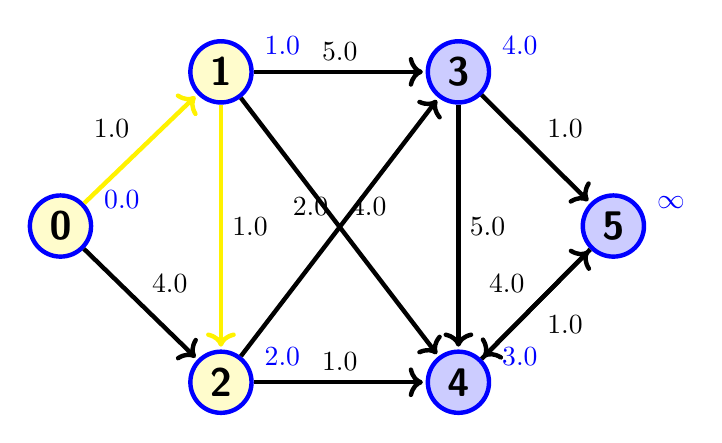
\begin{tikzpicture}[shorten >=1pt, auto, node distance=3cm, ultra thick,
        node_style/.style={circle,draw=blue,fill=blue!20!,font=\sffamily\Large\bfseries},
        selected_node_style/.style={circle,draw=blue,fill=yellow!20!,font=\sffamily\Large\bfseries},
        edge_style/.style={draw=black, ultra thick,->},
        selected_edge_style/.style={draw=yellow, ultra thick,->}]
        
        \node [selected_node_style,label={[text=blue]10:$0.0$}](n1) at (3.471,3.511) {0};
    
        \node [selected_node_style,label={[text=blue]10:$1.0$}](n2) at (5.509,5.469) {1};
    
        \node [selected_node_style,label={[text=blue]10:$2.0$}](n3) at (5.509,1.527) {2};
    
        \node [node_style,label={[text=blue]10:$4.0$}](n4) at (8.525,5.469) {3};
    
        \node [node_style,label={[text=blue]10:$3.0$}](n5) at (8.525,1.527) {4};
    
        \node [node_style,label={[text=blue]10:$\infty$}](n6) at (10.493,3.511) {5};
    
        \draw [edge_style] (n5) edge node{4.0} (n6);
    
        \draw [edge_style] (n6) edge node{1.0} (n5);
    
        \draw [selected_edge_style] (n2) edge node{1.0} (n3);
    
        \draw [edge_style] (n1) edge node{4.0} (n3);
    
        \draw [edge_style] (n4) edge node{1.0} (n6);
    
        \draw [edge_style] (n2) edge node{4.0} (n5);
    
        \draw [edge_style] (n3) edge node{2.0} (n4);
    
        \draw [selected_edge_style] (n1) edge node{1.0} (n2);
    
        \draw [edge_style] (n2) edge node{5.0} (n4);
    
        \draw [edge_style] (n3) edge node{1.0} (n5);
    
        \draw [edge_style] (n4) edge node{5.0} (n5);
    
        \end{tikzpicture}
    
            \end{center}
            \end{frame}
        
            \begin{frame}
            \frametitle{Dijkstra's Algorithm : Iteration 4 }
            \begin{center}
            
        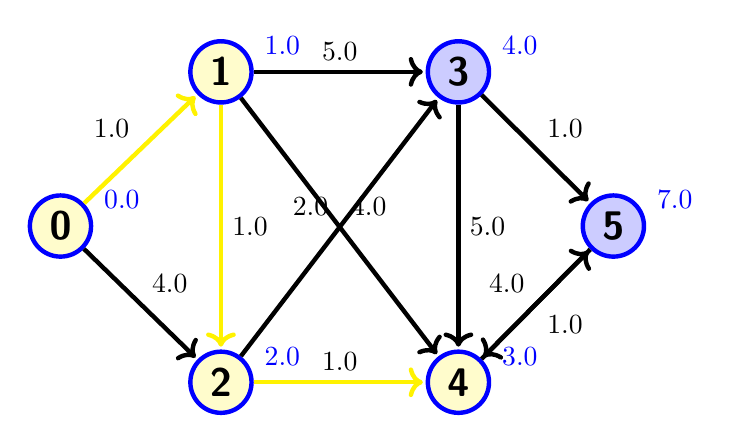
\begin{tikzpicture}[shorten >=1pt, auto, node distance=3cm, ultra thick,
        node_style/.style={circle,draw=blue,fill=blue!20!,font=\sffamily\Large\bfseries},
        selected_node_style/.style={circle,draw=blue,fill=yellow!20!,font=\sffamily\Large\bfseries},
        edge_style/.style={draw=black, ultra thick,->},
        selected_edge_style/.style={draw=yellow, ultra thick,->}]
        
        \node [selected_node_style,label={[text=blue]10:$0.0$}](n1) at (3.471,3.511) {0};
    
        \node [selected_node_style,label={[text=blue]10:$1.0$}](n2) at (5.509,5.469) {1};
    
        \node [selected_node_style,label={[text=blue]10:$2.0$}](n3) at (5.509,1.527) {2};
    
        \node [node_style,label={[text=blue]10:$4.0$}](n4) at (8.525,5.469) {3};
    
        \node [selected_node_style,label={[text=blue]10:$3.0$}](n5) at (8.525,1.527) {4};
    
        \node [node_style,label={[text=blue]10:$7.0$}](n6) at (10.493,3.511) {5};
    
        \draw [edge_style] (n5) edge node{4.0} (n6);
    
        \draw [edge_style] (n6) edge node{1.0} (n5);
    
        \draw [selected_edge_style] (n2) edge node{1.0} (n3);
    
        \draw [edge_style] (n1) edge node{4.0} (n3);
    
        \draw [edge_style] (n4) edge node{1.0} (n6);
    
        \draw [edge_style] (n2) edge node{4.0} (n5);
    
        \draw [edge_style] (n3) edge node{2.0} (n4);
    
        \draw [selected_edge_style] (n1) edge node{1.0} (n2);
    
        \draw [edge_style] (n2) edge node{5.0} (n4);
    
        \draw [selected_edge_style] (n3) edge node{1.0} (n5);
    
        \draw [edge_style] (n4) edge node{5.0} (n5);
    
        \end{tikzpicture}
    
            \end{center}
            \end{frame}
        
            \begin{frame}
            \frametitle{Dijkstra's Algorithm : Iteration 5 }
            \begin{center}
            
        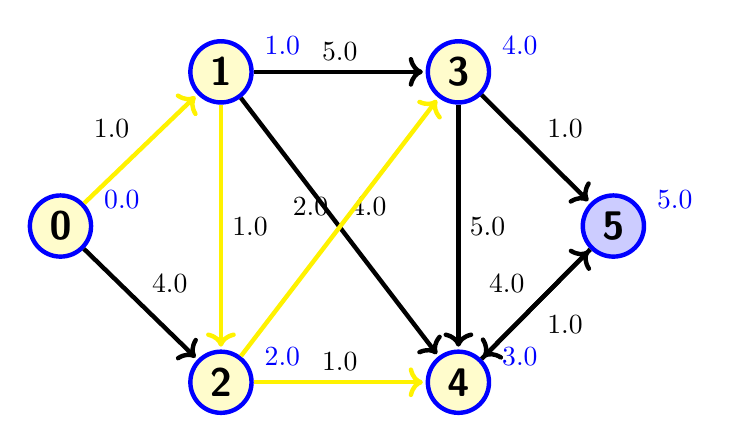
\begin{tikzpicture}[shorten >=1pt, auto, node distance=3cm, ultra thick,
        node_style/.style={circle,draw=blue,fill=blue!20!,font=\sffamily\Large\bfseries},
        selected_node_style/.style={circle,draw=blue,fill=yellow!20!,font=\sffamily\Large\bfseries},
        edge_style/.style={draw=black, ultra thick,->},
        selected_edge_style/.style={draw=yellow, ultra thick,->}]
        
        \node [selected_node_style,label={[text=blue]10:$0.0$}](n1) at (3.471,3.511) {0};
    
        \node [selected_node_style,label={[text=blue]10:$1.0$}](n2) at (5.509,5.469) {1};
    
        \node [selected_node_style,label={[text=blue]10:$2.0$}](n3) at (5.509,1.527) {2};
    
        \node [selected_node_style,label={[text=blue]10:$4.0$}](n4) at (8.525,5.469) {3};
    
        \node [selected_node_style,label={[text=blue]10:$3.0$}](n5) at (8.525,1.527) {4};
    
        \node [node_style,label={[text=blue]10:$5.0$}](n6) at (10.493,3.511) {5};
    
        \draw [edge_style] (n5) edge node{4.0} (n6);
    
        \draw [edge_style] (n6) edge node{1.0} (n5);
    
        \draw [selected_edge_style] (n2) edge node{1.0} (n3);
    
        \draw [edge_style] (n1) edge node{4.0} (n3);
    
        \draw [edge_style] (n4) edge node{1.0} (n6);
    
        \draw [edge_style] (n2) edge node{4.0} (n5);
    
        \draw [selected_edge_style] (n3) edge node{2.0} (n4);
    
        \draw [selected_edge_style] (n1) edge node{1.0} (n2);
    
        \draw [edge_style] (n2) edge node{5.0} (n4);
    
        \draw [selected_edge_style] (n3) edge node{1.0} (n5);
    
        \draw [edge_style] (n4) edge node{5.0} (n5);
    
        \end{tikzpicture}
    
            \end{center}
            \end{frame}
        
            \begin{frame}
            \frametitle{Dijkstra's Algorithm : Iteration 6 }
            \begin{center}
            
        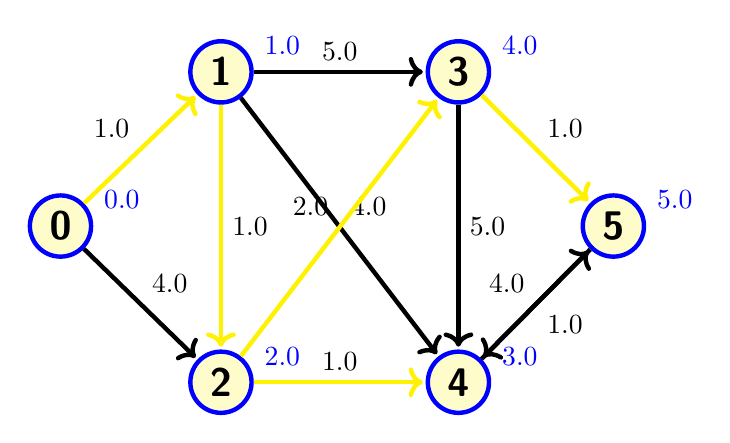
\begin{tikzpicture}[shorten >=1pt, auto, node distance=3cm, ultra thick,
        node_style/.style={circle,draw=blue,fill=blue!20!,font=\sffamily\Large\bfseries},
        selected_node_style/.style={circle,draw=blue,fill=yellow!20!,font=\sffamily\Large\bfseries},
        edge_style/.style={draw=black, ultra thick,->},
        selected_edge_style/.style={draw=yellow, ultra thick,->}]
        
        \node [selected_node_style,label={[text=blue]10:$0.0$}](n1) at (3.471,3.511) {0};
    
        \node [selected_node_style,label={[text=blue]10:$1.0$}](n2) at (5.509,5.469) {1};
    
        \node [selected_node_style,label={[text=blue]10:$2.0$}](n3) at (5.509,1.527) {2};
    
        \node [selected_node_style,label={[text=blue]10:$4.0$}](n4) at (8.525,5.469) {3};
    
        \node [selected_node_style,label={[text=blue]10:$3.0$}](n5) at (8.525,1.527) {4};
    
        \node [selected_node_style,label={[text=blue]10:$5.0$}](n6) at (10.493,3.511) {5};
    
        \draw [edge_style] (n5) edge node{4.0} (n6);
    
        \draw [edge_style] (n6) edge node{1.0} (n5);
    
        \draw [selected_edge_style] (n2) edge node{1.0} (n3);
    
        \draw [edge_style] (n1) edge node{4.0} (n3);
    
        \draw [selected_edge_style] (n4) edge node{1.0} (n6);
    
        \draw [edge_style] (n2) edge node{4.0} (n5);
    
        \draw [selected_edge_style] (n3) edge node{2.0} (n4);
    
        \draw [selected_edge_style] (n1) edge node{1.0} (n2);
    
        \draw [edge_style] (n2) edge node{5.0} (n4);
    
        \draw [selected_edge_style] (n3) edge node{1.0} (n5);
    
        \draw [edge_style] (n4) edge node{5.0} (n5);
    
        \end{tikzpicture}
    
            \end{center}
            \end{frame}
        

        \end{document}
    
